\chapter{Introduzione}

\section{Modello Standard}
Il Modello Standard (SM) è la teoria che ad oggi descrive meglio la fenomenologia delle interazioni tra particelle. Questa teoria, formulata nella seconda metà del novecento riesce a descrivere tre delle quattro interazioni fondamentali: interazione elettromagnetica, interazione debole e interazione forte, mentre ad oggi non esiste una estensione della teoria che comprenda l'interazione gravitazionale.


\begin{figure}
\centering
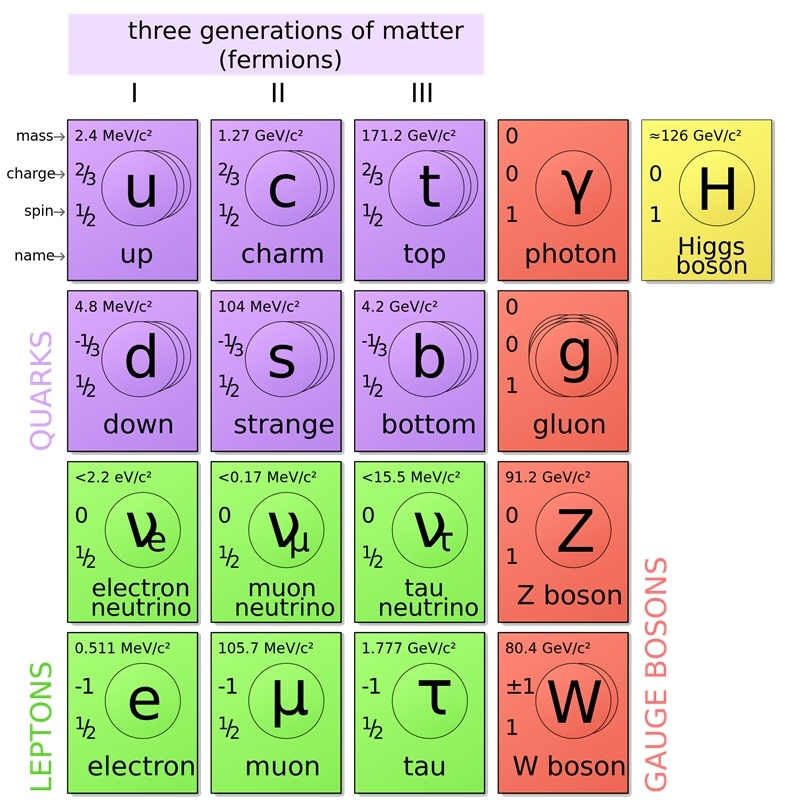
\includegraphics[scale=0.3]{Immagini/SM}
\caption{Particelle elementari del Modello Standard.}
\label{fig:SM}
\end{figure}

Questo modello)= descrive la materia come composta da due tipi di particelle, entrambe con spin semintero dunque fermioni, leptoni e quark:

\begin{itemize}
\item I leptoni hanno carica elettrica intera e quelli conosciuti sono 6, sono suddivisi in tre generazioni di doppietti con massa crescente. ogni doppietto è costituito da una particella con carica $Q=-1$ ($e$, $\mu$, $\tau$) che ha interazioni elettrodeboli, e da una particella neutra chiamata appunto neutrino ($\nu_e$, $\nu_{\mu}$, $\nu_{\tau}$) che dunque interagirà solo debole.

\item Analogamente ai leptoni i quark sono organizzati in doppietti, in questo caso però la carica è frazionaria e per ciascun doppietto ogni particella ha carica $Q=2/3$ ($u$, $t$, $c$), l'altra invece ha $Q=-1/3$ ($d$, $s$, $b$). I quark interagiscono sia elettrodebole che forte, quest'ultima interazione è alla base della formazione di stati legati chiamati adroni, come ad esempio neutrone e protone.
\end{itemize}

Ad ognuna di queste particelle corrisponde una antiparticella che ha i numeri quantici opposti ma stessa massa e spin. Oltre alle antiparticelle il Modello Standard prevede l'esistenza di bosoni: i bosoni di gauge ed il bosone di Higgs. 
Nel MS le forze sono espressioni di particolari simmetrie della teoria, ognuna delle quali viene mediata da particolari bosoni:

\begin{itemize}
\item Il fotone, responsabile della mediazione dell'interazione elettromagnetica.

\item I bosoni $W^{\pm}$ e il bosone $Z$, mediatori dell'interazione debole, un'esempio in cui entra in gioco questa forza è il decadimento $\beta$. Questi bosoni, al contrario di fotone e gluoni, sono massivi, circa $80 GeV$ e $91 GeV$ rispettivamente.

\item I gluoni, mediatori dell'interazione forte.
\end{itemize}

Come detto precedentemente la forza gravitazionale non è descritta dal MS, ma risulta essere trascurabile nelle interazione tra particelle, in quanto la sua intensità, paragonata a quella delle altre tre forze, è vari ordini di grandezza inferiore. Nel MS le interazioni sono descritte come manifestazioni di simmetrie della Lagrangiana. 
Queste simmetrie non ammettono termini di massa nella teoria, poiché questo porterebbe alla violazione delle
simmetrie di gauge. Tuttavia, attraverso un meccanismo di rottura spontanea della
simmetria, è possibile includere bosoni massivi aggiungendo alla teoria un ulteriore bosone, il bosone di Higgs. 
Attraverso il meccanismo di Higgs viene introdotta anche la massa dei fermioni, senza però predirne il valore.


\section{LHC e l'esperimento CMS}
CMS (Compact Muon Solenoid) è uno dei principali esperimenti condotti al CERN di Ginevra ad LHC (Large Hadron Collider), come lo sono anche ALICE, ATLAS e  LHCb. 

\begin{figure}
\centering
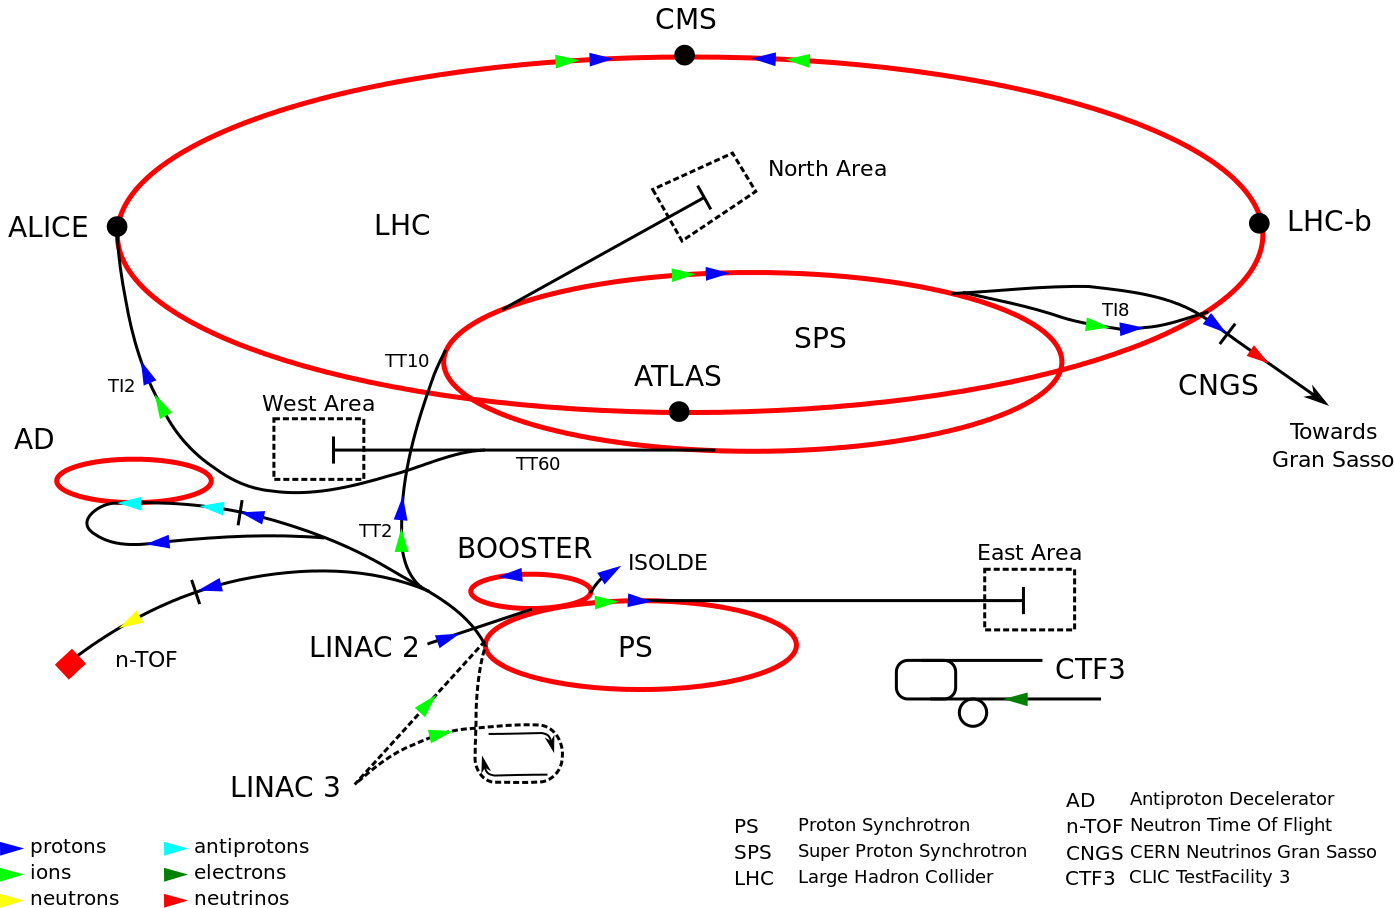
\includegraphics[scale=0.25]{Immagini/LHC}
\caption{Schema di preaccelerazione e accelerazione di LHC.}
\label{fig:LHC}
\end{figure}

Lo scopo di questi esperimenti è lo studio del Modello Standar e la ricerca di conferme sperimentali ai modelli teorici proposti. Questi esperimenti sono posti nei punti dell'acceleratore in cui i fasci di particelle si  incontrano interagendo e producendo eventi, che sono quindi registrati dall'esperimento per poi essere analizzati in seguito.
LHC è il più grande acceleratore di particelle mai costruito collocato in un anello sotterraneo di 27 km nella regione di Ginevra in sostituzione del precedente acceleratore, il LEP (Large Electron-Positron Collider).
LHC è stato concepito in modo da avere due anelli separati con campo magnetico opposto, al contrario del LEP dove venivano usati elettroni per un fascio e positroni per l'altro, che avendo carica opposta possono condividere la stessa beam pipe con lo stesso campo magnetico ruotando in senso opposto. 
Questa caratteristica insieme a tante altre (energie nel centro di massa elevate alto rate...) ha portato ad una grande innovazione tecnologica ed ha aumentato considerevolmente la complessità della macchina. 

Attualmente l'energia nel centro di massa $\sqrt{s}=14$ TeV, il motivo di una così alta energia è spiegato con la necessità di indagare processi fisici i cui effetti sono maggiormente visibili se si è sopra una certa scala di energia. Un esempio è il Bosone di Higgs scoperto nel 2012, la cui massa è circa $125$ $GeV$.

L'accelerazione dei protoni è graduale, i protoni ottenuti da idrogeno gassoso sono inizialmente accelerati attraverso un acceleratore lineare, LINAC2, figura \ref{fig:LHC}. Successivamente i protoni sono iniettati nel Proton Sybchroton Booster (PSB) che aumenta l'energia fino a $1.4$ $GeV$, in seguito grazie al Proton Synchrotron raggiungono i $25$ $GeV$. 
Inoltre in queste fasi i protoni vengono raggruppati in pacchetti distanti temporalmente $25$ $ns$(ovvero hanno una frequenza di $40 MHz$, frequenza massima a cui LHC opera). 
Infine vengono accelerati fino ad energie di $450 GeV$ nel Super Proton Synchrotron (SPS) prima di essere iniettati nei due anelli di LHC che li accelera prima di farli collidere nei punti in cui sono collocati gli esperimenti:

\begin{itemize}
\item ALICE (A Large Ion Collider Experiment), esperimento che studia un nuovo stato della materia, il quark-gluon plasma, prodotto nelle collisioni di ioni pesanti.

\item CMS (Compact Muon Solenoid) e ATLAS (A Toroidal LHC ApparatuS), entrambi costruiti con lo scopo di investigare il più ampio spettro di fisica possibile. Grazie a loro è stata possibile la scoperta del bosone di Higgs. I due esperimenti hanno gli stessi obbiettivi, ma sono stati costruiti con desing differenti al fine di essere indipendenti nella ricerca e studio dei processi di interazione che avvengono durante le collisioni tra due protoni.

\item LHCb (LHC beauty), esperimento che studia la fisica degli adroni contenenti il quark b e la violazione di CP (coniugazione di Carica e Parità) nelle interazioni elettrodeboli.
\end{itemize}

Altri esperimenti presenti ad LHC, ma di dimensioni minori sono TOTEM e LHCf:

\begin{itemize}
\item TOTEM (TOTal Elastic and diffractive cross section Measurement), misura accuratamente la luminosità di LHC e ha come fine lo studio delle interazioni in cui i protoni escono con piccoli angoli.

\item LHCf (LHC forward), è composto da due rivelatori che sono posizionati a $140$ m dal punto di collisione di ATLAS. Studia i prodotti delle collisioni a grande rapidità e alt energia, con lo scopo di modellizzare il comportamento dei raggi cosmici primari.
\end{itemize}


\subsubsection{Fisica degli acceleratori}

Nei tubi in cui circolano i due fasci la pressione di vuoto è di $10^{-13}$ $atm$, per evitare che i protoni urtino molecole di gas interagendo. 
Essendo LHC un acceleratore circolare è necessario un sofisticato sistema di curvatura, è perciò necessario un campo magnetico ortogonale  all'anello per curvare i fasci di particelle. 
Il campo necessario per deflettere una particella di carica unitaria è dato da:
\begin{equation}
P[GeV]= 0.3 \cdot B[T] \cdot r[m]
\end{equation}
dove $B$ è il campo magnetico, $r$ il raggio di curvatura e $P$ l'impulso della particella. Dati i parametri di LHC ($r= 4 \cdot 10^3 m$ e $P=7 TeV$) si ottiene un campo $B$ che in media è pari a $5.8 T$. Per ottenere un tale campo è stato necessario l'utilizzo di dipoli magnetici superconduttori, il che ha rappresentato una importante sfida tecnologica per la progettazione di LHC. L'impiego di magneti superconduttivi è necessario per la generazione di campi magnetici così elevati. Ciò avviene a temperature molto basse, dell'ordine dei 2 K, temperatura mantenuta grazie ad un complesso sistema di criogena.

Al fine di ottenere risultati con un'ampia statistica ed una buona precisione è importante per un acceleratore avere alta luminosità, questo parametro corrisponde al numero di collisioni prodotte per unità di area e tempo e può essere espressa in funzione del rate R di particelle e della sezione d'urto $\sigma$ 
\begin{equation}
L=\frac{R}{\sigma}
\end{equation}
Un altro modo di esprimere la luminosità è metterla in funzione delle variabili ch caratterizzano il fascio:
\begin{equation}
L = f \frac{N_1 N_2}{4 \pi \sigma_x \sigma_y}
\end{equation}
con $N_1$ $N_2$ numerodi protoni per bunch, f frequenza collisioni e $4\pi \sigma_x \sigma_y =A$ area efficacie. Alle vlte è anche utile parlare di luminosità integrata $L_{int}=\int L dt$ che permette di ottenere la relazione tra numero di eventi e sezione d'urto:
\begin{equation}
N=\sigma L_{int}
\end{equation}

Attraverso la scelta di sostituire il collisionatore leptonico LEP con uno adronico
come LHC si sono ottenuti due vantaggi fondamentali: 
\begin{itemize}
\item A parità di dimensioni l'energia raggiunta nel centro di massa è maggiore, poichè l'energia persa per radiazione di sincrotrone scala come la potenza quarta della massa della particella. Dunque a parità di energia la perdità per un protone è circa $10^{13}$ volte minore di quella di un elettrone.

\item La struttura non elementare dei protoni permette di avere uno spettro energetico più ampio, senza dover cambiare i parametri del fascio. Questo perchè i protoni al contrario degli elettroni, che sono particelle elementari, hanno una struttura interna e nella collisione l'interazione coinvolge una coppia di partoni che trasportano solo una frazione  casuale dell'impulso iniziale del protone.
\end{itemize}

\section{HL-LHC}
Il progetto di upgrade HL-LHC, formalmente approvato nel giugno 2016 dal CERN, permettera di ampliare il campo di indagine di fenomeni fisici rari all'interno del Modello Standard ed anche di ricercare processi di nuova fisica BSM (Beyond Standard Model). Questa fase di alta luminosità permetterà a CMS di raggiungere precisioni del per cento su misure di accoppiamento del bosone di Higgs prese nel Run 1. Inoltre nella fase HL-LHC ci si aspetta siano possibili misure come l'accoppiamente trilineare di bosoni di Higgs. 
I processi deboli di scattering di bosoni vettori sono profondamente legati alla rottura della simmetria elettro bedole e dal punto di vista della misura sono una sfida, in quanto le sezioni d'urto sono piccole e i fondi irriducibili sono dominanti. 

L'aumento di luminosità ad LHC permetterrà lo studio di questi canali, per far ciò  l'upgrade di LHC sarà accompagnato da un programma di adeguamento dell'esperimento CMS, al fine di mantenere alte le prestazioni del rivelatore (efficienza, risoluzione,reiezione di processi di fondo...) nonostante l'aumento di radiazione e le più difficili condizioni operative, come ad esempio pile-up più frequente.
In figura \ref{HL-LHC} è mostrato un prospetto della scaletta dei tempi di LHC dal 2015 in poi. Il Run 2 continuerà fino alla fine del 2018, quando inizierà il Long Shutdown 2 (LS2) e dopo cui si avrà la fase di Run 3.  Entro il 2022 si stima sarà raccolta una luminosità integrata di circa $300 fb^{-1}$. 
Durante il Long Shutdown 3 (LS3), programmata dal 2022 fino alla metà del 2024, saranno eseguiti gli aggiornamenti principali di LHC e degli esperimenti per la fase di alta luminosità.

\subsection{Obiettivi}
\begin{figure}
\centering
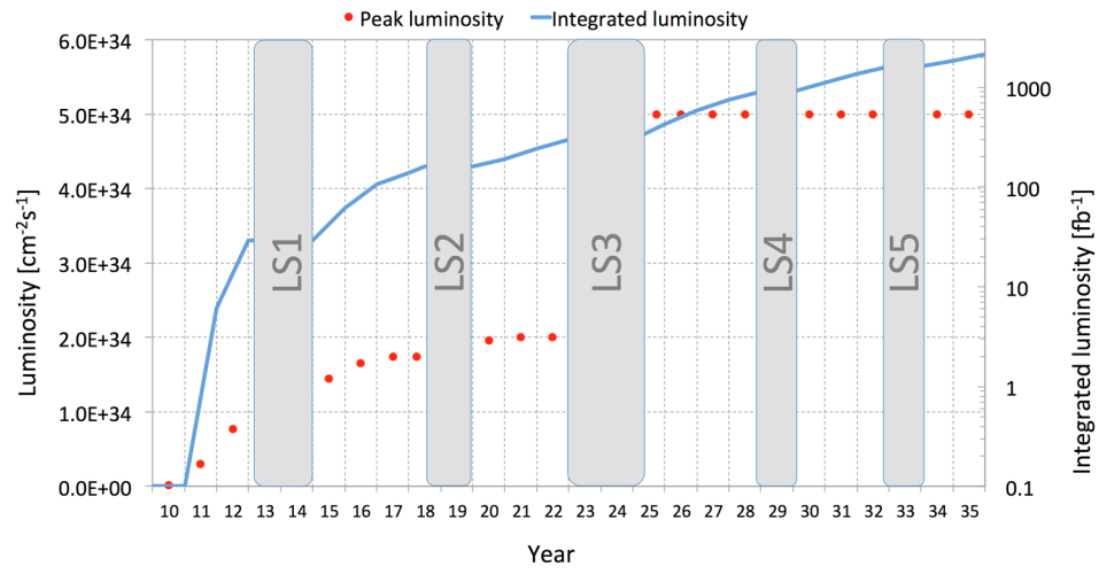
\includegraphics[scale=.35]{Immagini/HL-LHC}
\caption{Projected LHC performance through 2035, showing preliminary dates for long shut downs of LHC and projected luminosities.reference LHCC P 008}
\label{HL-LHC}
\end{figure}

L'idea di aumentare la luminosità di LHC oltre quella decisa nel progetto originale è antecedente alla messa in opera del progetto. Eventuali modifiche importanti allla macchina e agli esperimenti possono essere reseguite solo con lunghi periodi di shut down in cui è possibile accedere al tunnel e alle caverne. Per questo motivo è stato deciso un piano temporale che intervalli periodi di presa dati (Run I, Run II etc.) e periodi in cui si ha uno spegnnimento completo per lunghi periodi (LS1, LS2, LS3). In figura \ref{HL-LHC} è possibile vedere la suddivisione temporale tra priodi di presa dati e periodi di spegnimento.
Run I è stato il periodo di presa dati dal 2011 al 2012. Nel primo periodo di stop LS1 LHC è stato modificato al fine di raggiungerer energie  nel centro di massa di 13 TeV, per poi arrivare gradualmente a 14 TeV. In questo momento siamo alla fine del Run II, e nell'esperimento CMS si  hanno una media di 25 interazioni per bunch, ciò vuol dire 25 vertici da ricostruire ogni 25 ns. Attreverso modifiche  e miglioramenti apportati nel LS1 e LS2 verrà aumentata la luminosità, questa parte del processo per l'esperimento CMS va sotto il nome di fase-I. Durente il periodo LS3  saranno invece sostituite vari parti degli esperimenti, che a causa del dannegggiamnto da radiazione saranno deteriorati e nello contemporaneamente verrano sostituiti i quadrupoli di fuocheggiamento con nuovi modelli capaci di incrementare la luminosità. 
Il periodo che seguira LS3 sarà chiamato fase II o HL-LHC (High Luminosity LHC). Nello scenario prefissato la lumiosità istantanea sarà di $5 \cdot 10 34 cm^{-2} s^{-1}$ con picchi di $2 \cdot 10 35 cm^{-2} s^{-1}$, in questo modo gli esperimenti saranno in grado di raccogliere una maggiore statistica con una luminosità di $300 fb^{-1}$ ogni anno per 10 anni(250 o 300)?????%at 5 × 10 34 cm − 2 s − 1 from a potential peak value of 2 × 10 35 cm − 2 s − 1 at the beginning of fills,
%and to deliver 250 fb − 1 per year for a further 10 years of operation. Under these conditions
In queste condizioni ci sarà una maggiore probabilità di sovrapposizione di interazioni (Pile Up), questa sarà la grande sfida, insieme alla gestione degli effetti di degradazione in cui incorreeranno i rivelatori a seguito delle maggiori dosi di radiazione assorbita. Sempre nella figura \ref{HL-LHC} è possibile vedere le proiezioni di luminosità di picco e luminosità integrata.
 
%The high luminosity period that follows LS3 with the upgraded LHC is referred to here as HL-LHC or Phase-II. The proposed operating scenario is to level the instantaneous luminosity
%at 5 × 10 34 cm − 2 s − 1 from a potential peak value of 2 × 10 35 cm − 2 s − 1 at the beginning of fills,
%and to deliver 250 fb − 1 per year for a further 10 years of operation. Under these conditions the event PU will rise substantially to become a major challenge for the experiments, and the performance degradation due to integrated radiation dose will need to be addressed. This Technical Proposal presents the CMS upgrade program for Phase-II. The schedule of beam operations and long shutdowns, together with projections of the peak and integrated luminosities, is shown in Fig. 1.9, and is, of course, subject to change.

\section{Esperimento CMS}
CMS è un esperimento ad ampio spettro che opera ad LHC, è installato un centinaio di metri sotto terra CMS nei pressi del paese Cessy, in Francia, tra il lago di Ginevra e il complesso dei monti Jura. Essendo ad ampio spettro i suoi rivelatori sono in grado di distinguere un gran numero di particelle $e$, $\mu$, $\tau$, $\gamma$ etc...
L'obiettivo principe di LHC è quella di indagare la natura della rottura spontanea della simmetria elettrodebole alla base di cui sta il meccanismo di Higgs. Lo studio sperimentale del meccanismo di Higgs consente inoltre di verificare la consistenza del Modello Standard a scale di energia dei TeV. Inoltre c'è la speranza di nuove scoperte che offrano indicazioni su teorie oltre al Modello Standard, come ad esempio Supersimmetrie o Extra Dimension.
Ad LHC vengono utilizzati anche fasci di ioni pesanti, che hanno energie 30 volte superiori ai precedenti acceleratori, permettendo così uno studio approfondito della QCD in condizioni estreme di temperatura, densità e frazioni di momento partonico. Con la luminosità ed energia nel centro di massa raggiungibili ad LHC un ampio spettro di fisica diventa accessibile, questo però vincola i vari esperimenti, compreso CMS a richieste stringenti sulle prestazioni e quindi sulla progettazione e messa in opera.
Con un'energia nel centro di massa di 14 TeV la sezione d'urto protone-protone è circa 100 mb, data la  luminosità questo porta a circa $10^9$ eventi al secondo, che grazie al processo di selezione online viene abbassato fino a 100 eventi al secondo, i quali vengono poi memorizzati per una successiva analisi. 
Ogni 25 ns vi è una nuova collisione tra bunch di particelle che con le sue circa 20 collisioni produce un alto numero di particelle che dovranno essere rivelate con l'attenzione a distinguerle le une dalle altre. Questo richiede un'alta segmentazione del rivelatore e una buona risoluzione tmporale , al fine di evitare effetti di pile-up. Il tutto cercando di ridurre il più possibile i volumi.
Inoltre dato l'alto flusso di particelle il rivelatore e l'elettronica di lettura devono essere in grado di resistere ad alti livelli di radiazione. Tutti questi motivi hanno  portato alla necessità di alti requisiti per il buon funzionamento dell'esperimento:
\begin{itemize}
\item Buona capacità di identificare i muoni e ottima risoluzione degli impulsi su ampio angolo.
\item Alta efficienza del tracciatore e buona risoluzione dei momenti di particelle cariche.
\item Buona risoluzione nella misura dell'energia elettromagnetica, copertura maggiore possibile di tutto l'angolo solido e ottima capacità di isolamento di fotoni e leptoni.
\item Buona risoluzione dell'energia transversa mancante (MET) e calorimetri adronici con coperture ampia dell'angolo solido e buona segmentazione.
\end{itemize}

Il sistema di coordinate adottato da CMS è tale che l'origine corrisponde al punto di collisione dei due fasci con asse y verticale orientato verso l'alto e asse x in direzione radiale verso il centro di LHC. L'angolo azimutale $\phi$ è misurato a partire dall'asse x e giace sul piano x-y e la coordinara radiale su questo piano è $r$. L'angolo polare $\theta$ è misurato dall'asse z. 

Per lo studio dei processi è utile itrodurre anche grandezze invarianti per trasformazioni di Lorentz come $\Delta y$ e $\Delta \eta$, dove y indica la rapidità e $\eta$ la pseudorapidità:
\begin{equation}
y= \dfrac{1}{2} ln\Big( \dfrac{E+p_z}{E-p_z}\Big)
\end{equation}

\begin{equation}
\eta = - ln \Big( tg\frac{\theta}{2}\Big)
\end{equation}
Infine la differenza nel bilancio dell'energia misurata sul piano trasverso è indicata come $E_T^{miss}$.


\subsection{Il rivelatore CMS}
CMS è un esperimento a simmetria cilindrica, ha un diametro di 15 m ed è lungo 21.6 m, per un peso complessivo di circa 12500 tonnellate. Lo scopo dell'esperimento è studiare una vasta gamma di processi fisici delle interazioni protone-protone, figura \ref{CMS}. 
\begin{figure}
\centering
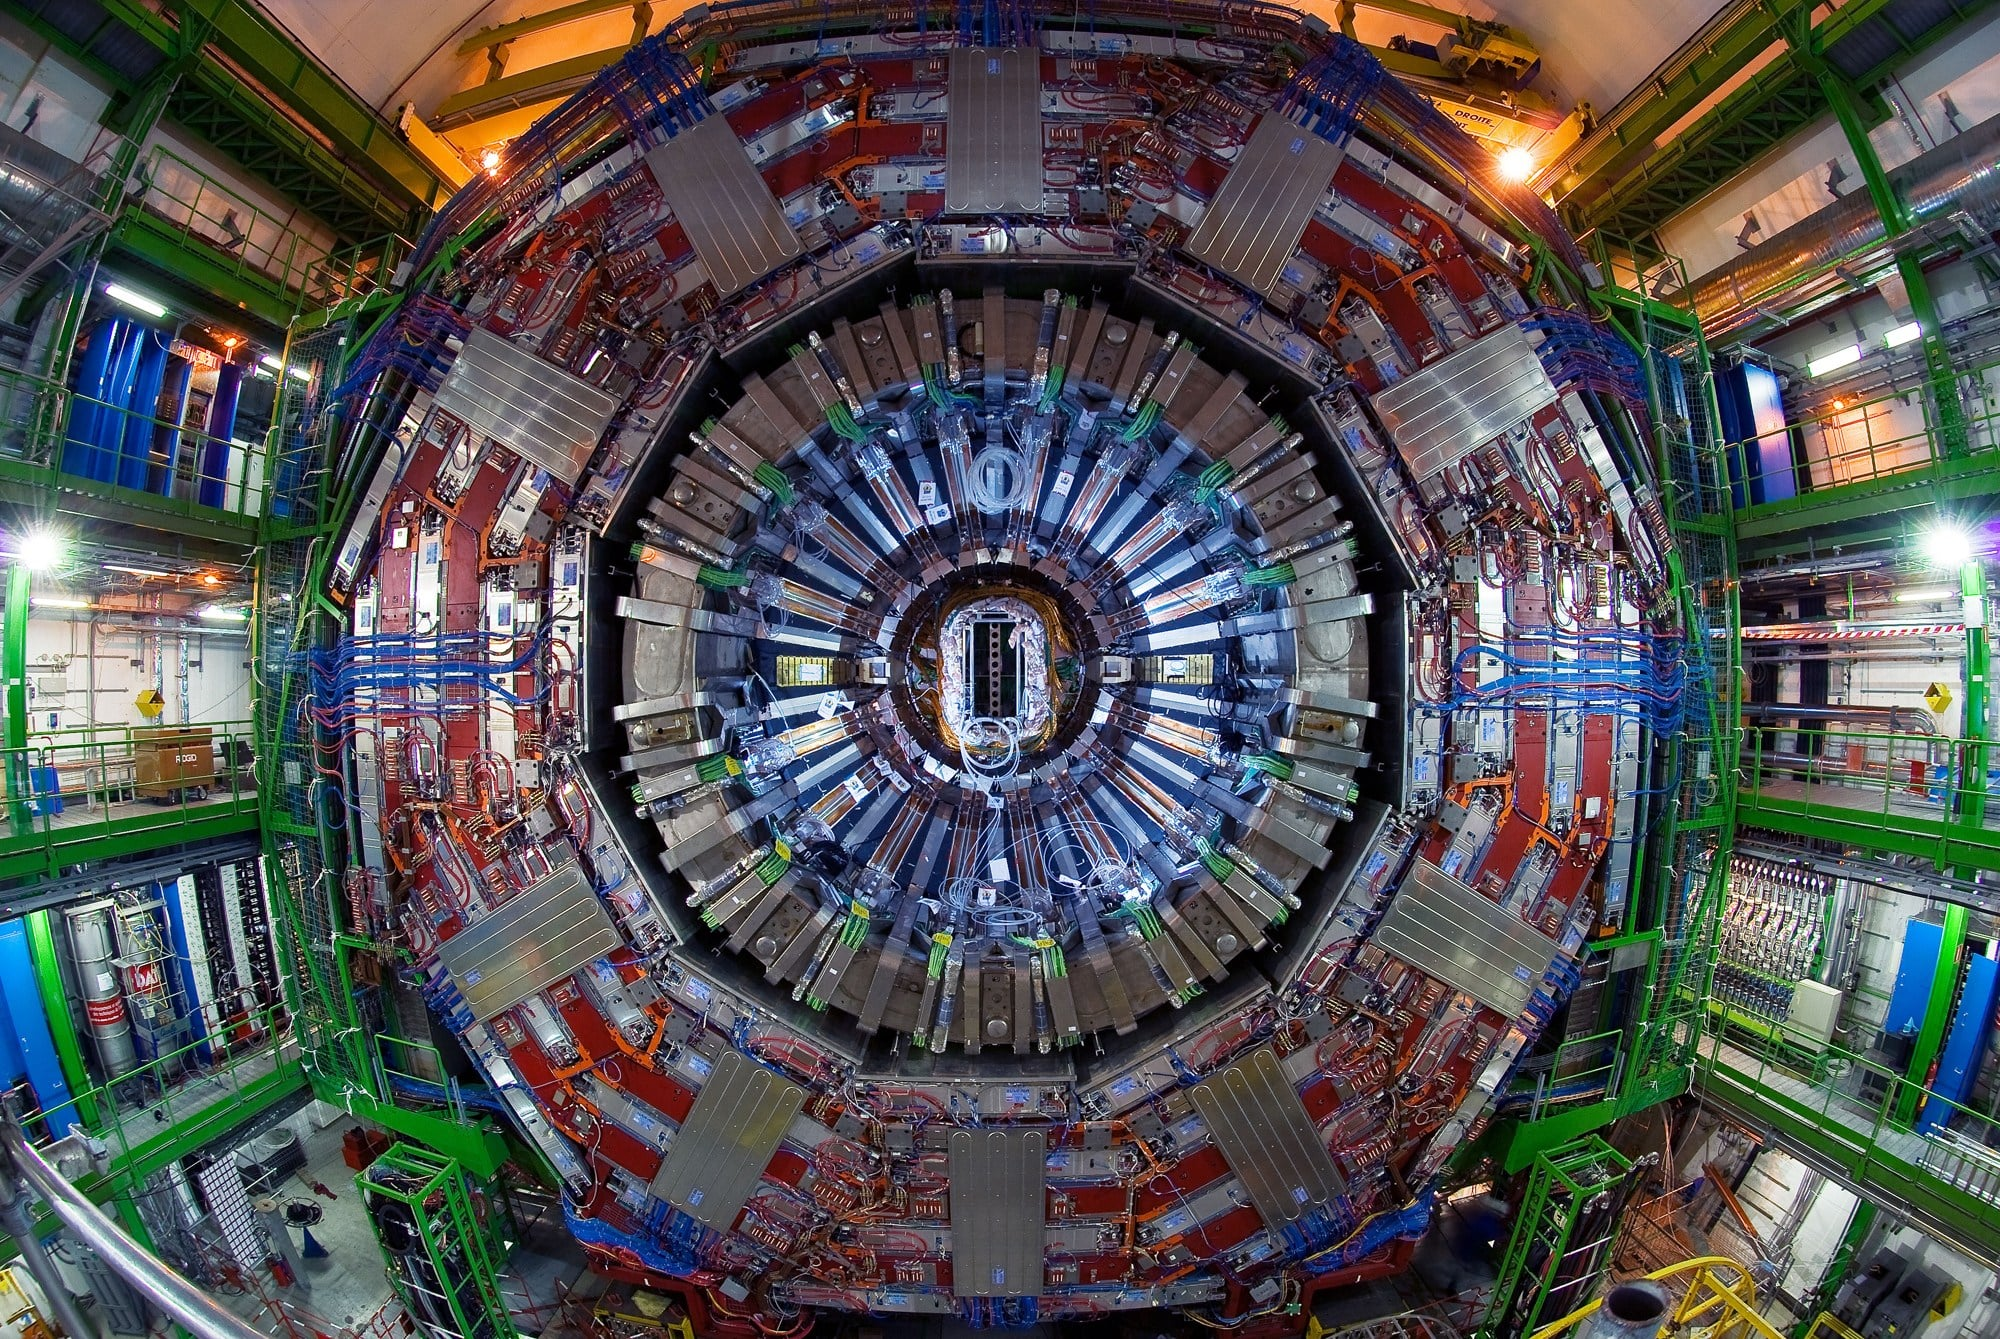
\includegraphics[scale=.2]{Immagini/CMS}
\caption{Vista frontale di CMS durante l'installazione del tracciatore.}
\label{CMS}
\end{figure}
Per questo motivo è composto da diversi tipi di rivelatori, disposti in modo concentrico rispetto al punto di collisione dei due fasci. 
La parte centrale di CMS è racchiusa in un solenoide superconduttivo lungo 13 metri e con un diametro di 6, capace di generare un campo di $3.8 T$, questo consente  di curvare abbastanza la traiettoria di tutte le particelle cariche e specialmente dei muoni, consentendo così di misurarne l'impulso trasverso. Il campo magnetico del solenoide si richiude su un giogo di ritorno in ferro, inframezzato al ferro del giogo sono posizionati i rivelatori di muoni. Ogni rivelatore di muoni consta di vari strati di Drift Tubes in allumnio (DT) sulla superficie cilindrica e cathode strip chamber (CSC) nelle regioni estreme che chiudono il rivelatore, dette endcap, a questi si aggiungono le resistive plate chamber (RPC). 
Nella parte interna del magnete è contenuto il tracciatore e i calorimetri. Per quanto riguarda il tracciatore la parte più interna è composta da 3 piani di rivelatori a pixel in  silicio, più esternamente sono stati installati 10 piani di rivelatori a microstrip di silicio. 
Sempre internamente al solenoide sono posti intorno al tracciatore i calorimetri elettomagnetici (ECAL) utilizza cristalli di tungstato di piombo ($PbWO_4$) con copertura in pseudorapidità fino a  $|\eta |< 3.0$. La luce di scintillazione viene letta a fotodiodi a valanga di silicio (APDs) e fototriodi a vuoto (VPTs) nelle regioni di endcup, dove il campo magnetico è basso. 
\begin{figure}
\centering
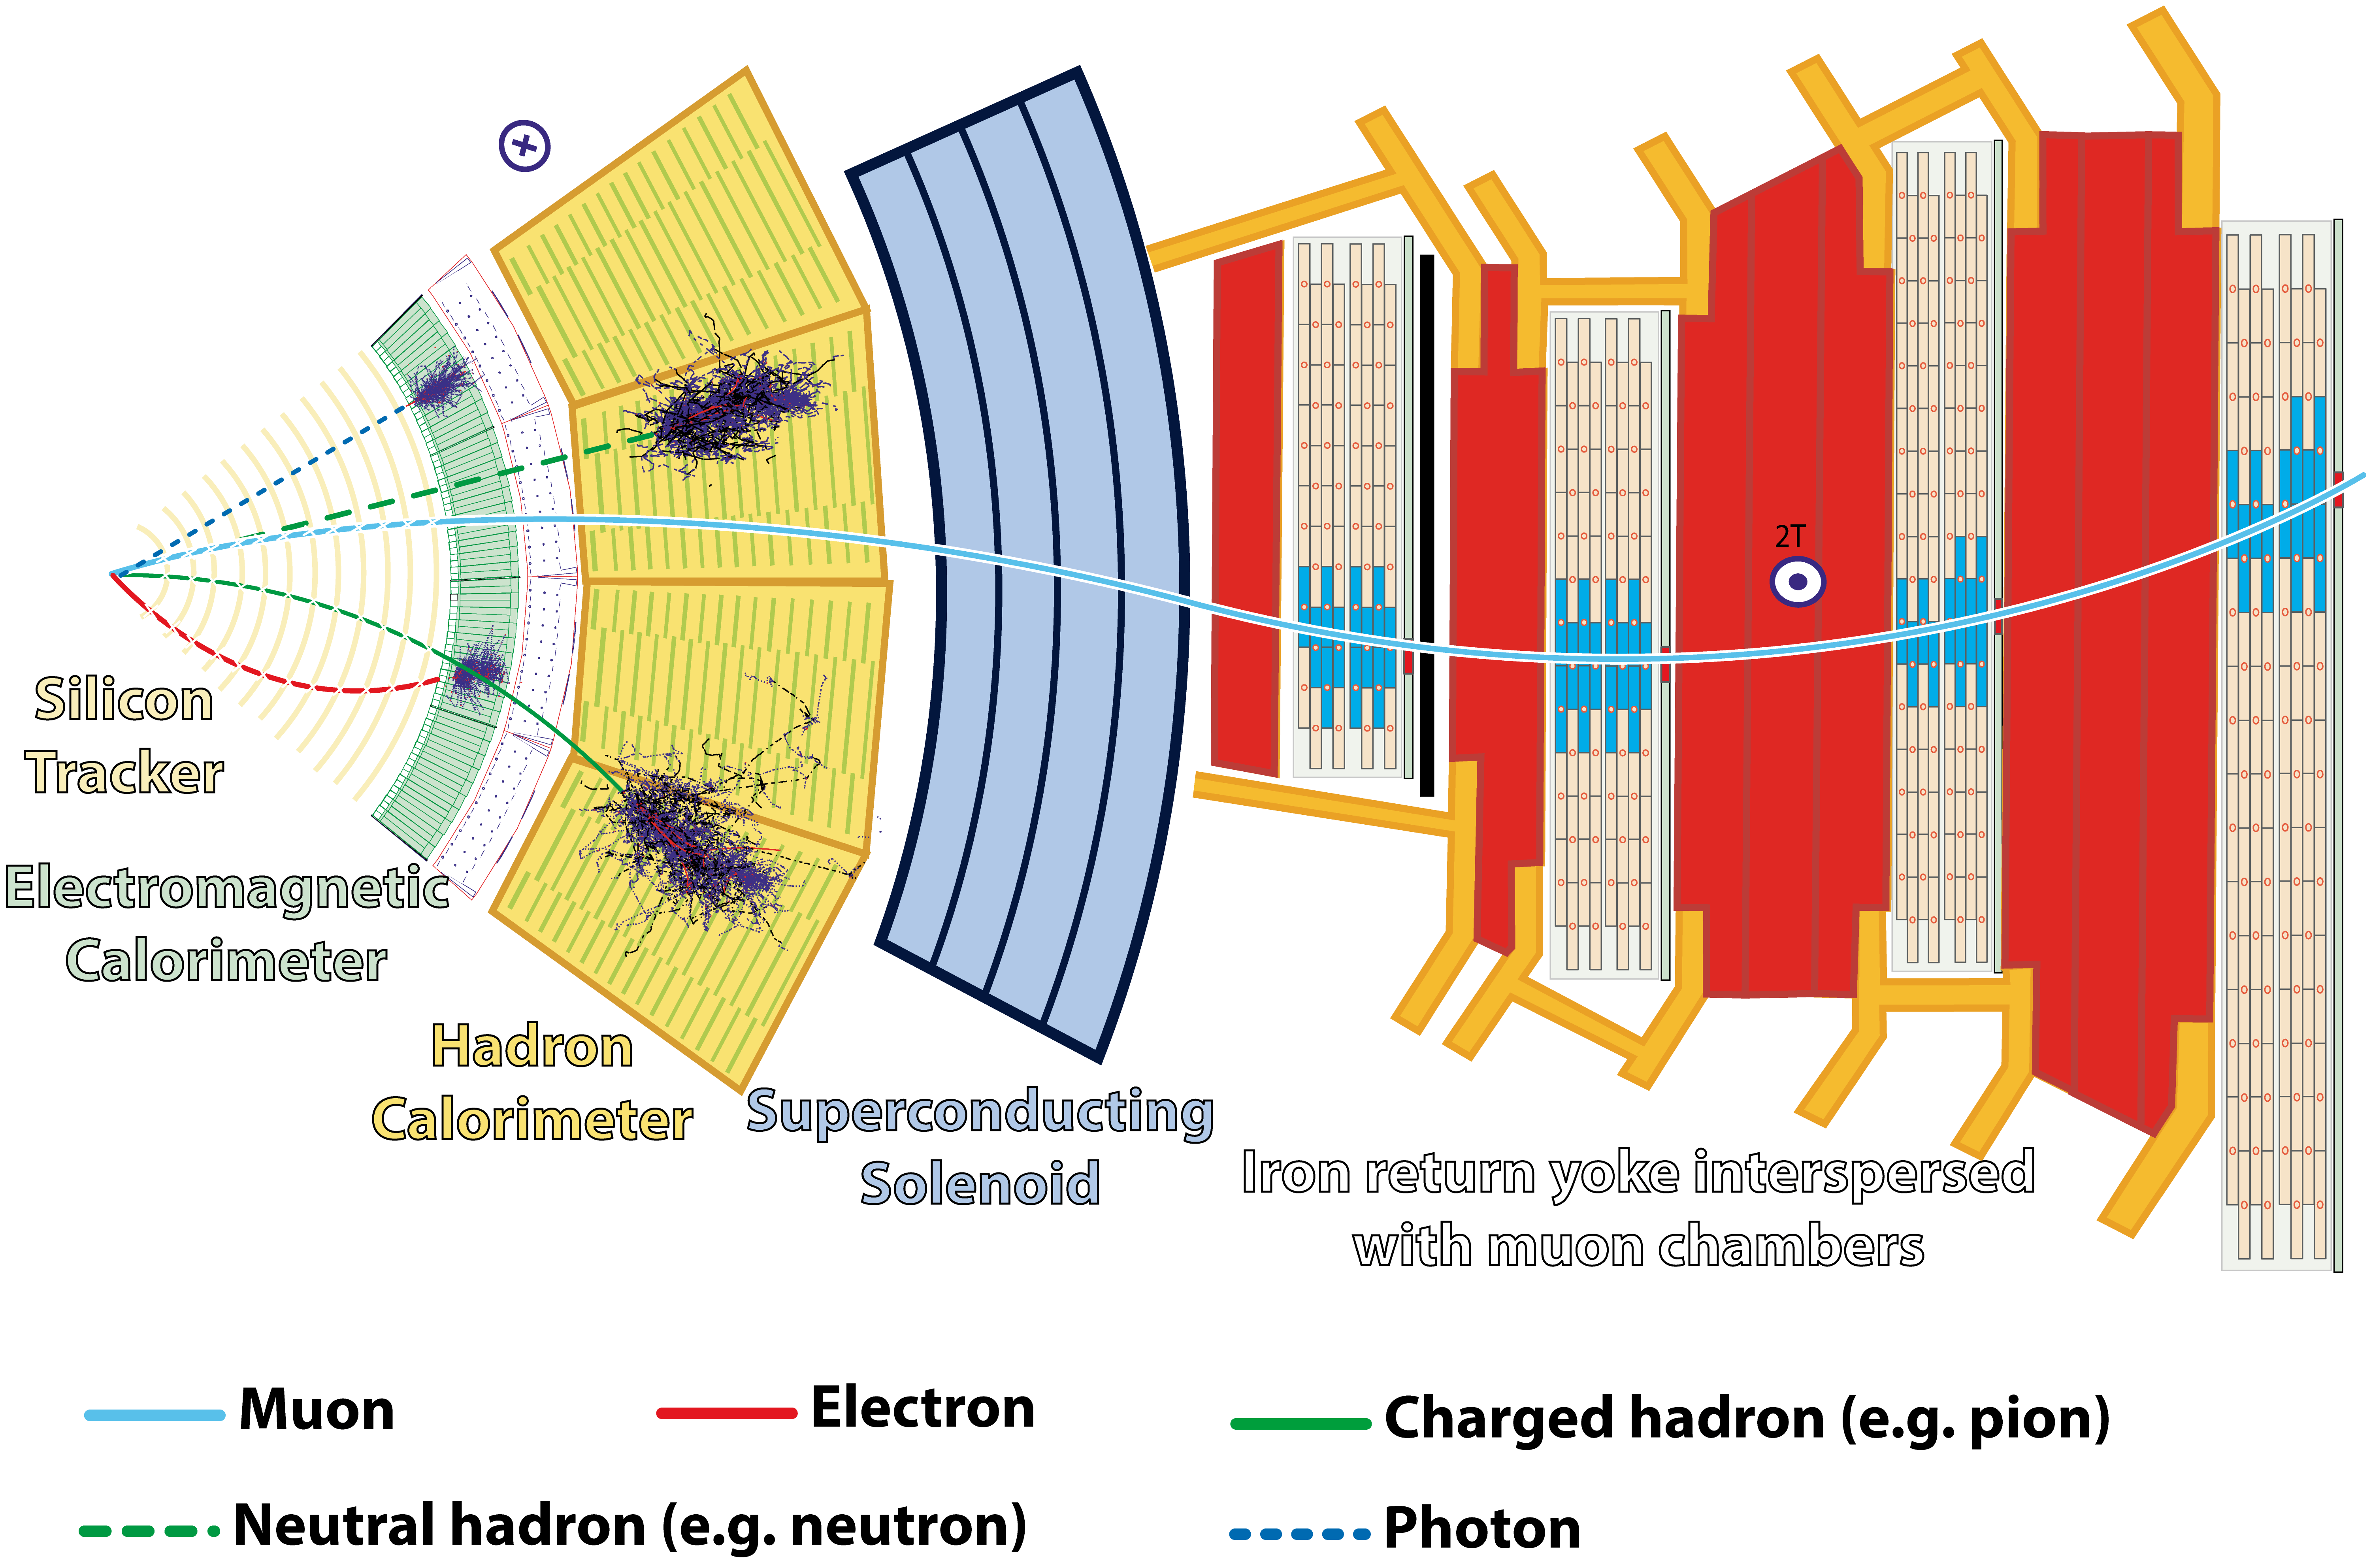
\includegraphics[scale=0.8]{Immagini/CMSbis}
\caption{Spaccato di CMS e risposta ai vari tipi di particella.}
\label{CMSbis}
\end{figure}
Le varie parti che compongono CMS, dall'interno verso l'esterno sono, figura \ref{CMSbis}:

\begin{itemize}
\item Tracciatore

\item Calorimetro elettromagnetico

\item Calorimetro adronico

\item Magnete superconduttore solenoidale

\item Camere a muoni

\end{itemize}

Questa struttura rispecchia la necessità di ricostruire con precisione gli eventi originati dalla collisione di particelle, che avvengono in rapida successione. CMS come anche gli altri esperimenti, può essere paragonato ad una gigantesca macchina fotografica che registra 40 milioni di foto al secondo (digitalizzando l'informazione di decine di milioni di sensori). 
La struttura a strati consente di avere rivelatori diversi in ogni strato, di cui i più interni sono meno densi, mentre i più esterni sono più densi. Questo perché il tracciatore non deve alterare l'energia delle particelle che poi sarà misurta nei calorimetri e per facilitare la ricostruzione delle tracce è importante evitare fenomeni di multiple scattering.

Le particelle che gli scienziati cercano di riprodurre nelle collisioni protone-protone hanno vite medie molto brevi, e decadono rapidamente in particelle più leggere. Dopo un processo di hard-scattering migliaia di queste particelle leggere sono generate elettroni, muoni, fotoni, ma anche protoni, neutroni etc. Tutte queste particelle attraversano i vari strati di cui è composto il rivelatore. 
Le informazioni raccolte vengono utilizzate per ricostruire l'evento di interazione, per  dedurre l'esistenza di nuove particelle pesanti....


Le traiettorie delle particelle cariche sono piegate dal campo magnetico, e il loro raggio di curvatura è utilizzata per calcolare il loro impulso: maggiore è la loro energia cinetica, minore è la curvatura. Un'altra componente importante di un rivelatore sono i calorimetri per misurare l'energia delle particelle (sia cariche che non). 
I calorimetri devono essere abbastanza grandi per assorbire anche le particelle più energetiche. Questi motivi fanno sì che gli esperimenti ad LHC siano così grandi. I rivelatori sono costruiti in modo il più possibile ermetico per raccogliere tutti i prodotti delle interazioni e poter ricostruire gli eventi. 
Combinando le informazioni di ogni strato del rivelatore è possibile determinare il tipo di particella che ha lasciato una data traccia.

Particelle cariche come elettroni, protoni e muoni, lasciano tracce ionizzando il materiale attraversato. Gli elettroni sono molto leggeri e perciò perdono energia velocemente, mentre i protoni penetrano più in profondità negli strati del rivelatore. I fotoni essendo neutri non rilasciano segnali nel tracciatore, ma nei calorimetri sono convertiti in elettroni e positroni e così ne viene misurata l'energia. 
L'energia dei neutroni viene invece misurata indirettamente, trasferiscono l'energia ai protoni, che poi sono misurati. I muoni insieme ai neutrini (che non vengono rivelati) sono i soli a raggiungere gli strati più esterni.


\begin{figure}
\centering
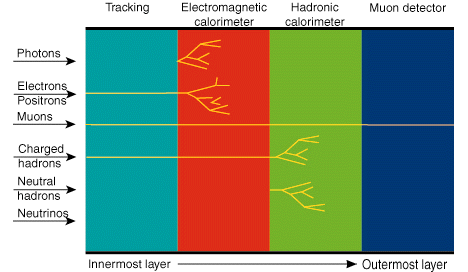
\includegraphics[scale=0.7]{Immagini/CMSinterazione}
\caption{Spaccato di CMS e risposta ai vari tipi di particella.}
\label{CMSinterazione}
\end{figure}

Ogni parte del rivelatore è connessa ad un sistema di lettura elettronico attraverso migliaia di cavi. Ogni volta che un segnale è raccolto, il sistema registra la sua posizione e l'istante in cui è stato raccolto, se il sistema di trigger decide che l'evento che ha generato Se tale segnale è di interesse, allora l'informazione è letta e portata all'esterno del rivelatore per essere utilizzata nelle analisi offline.
Ci sono differenti criteri per selezionare un evento potenzialmente di interesse, in questo modo la mole enorme di eventi registrati in un secondo viene ridotta a poche centinaia, che poi verranno analizzate in dettaglio.


\subsection{Tracciatore}
Il tracciatore al silicio  è il rivelatore più vicino al punto dove collidono i due fasci. 
\begin{figure}
\centering
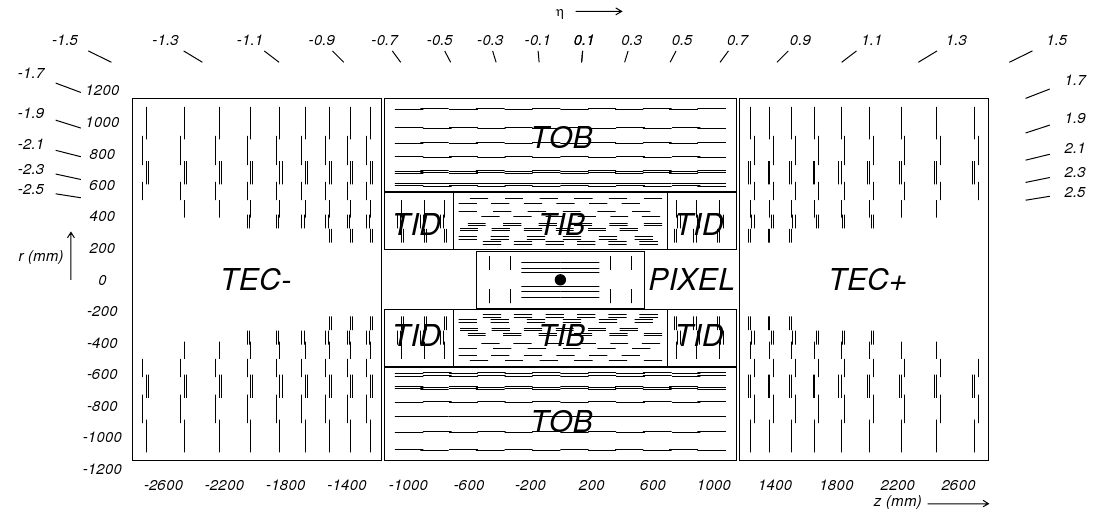
\includegraphics[scale=0.35]{Immagini/CMStracker}
\caption{Tracciatore CMS visto nel piano $rz$. Ogni linea nel tracciatore a strip rappresenta un rivelatore a strip, mentre nel rivelatore a pixel ogni linea rappresenta la struttura su cui i rivelatori sono montati.}
\label{CMStracker}
\end{figure}
Lo scopo è ricostruire , con la maggior precisione possibile, le traiettorie delle particelle cariche, identificando vertici primari e secondari. La composizione interna del tracciatore è mostrata in figura \ref{CMStracker}. Il raggio esterno è circa 110 cm e la lunghezza totale circa 540 cm.

Nella zona centrale (barrel) e più interna vi è il rivelatore di vertice a pixel, con tre strati distanti 4, 7 e 11 cm dall'asse dei fasci. La dimensione dei pixel è $100x150$ $\mu m^2$. Più esternamente ci sono rivelatori a microstrip tra 20 e 110 cm. Le parti laterali, dette endcap, sono invece costituite da 2 piani a pixel e 9 a microstrip. La parte di microstrip è divisa in due parti Inner Barrel e Outer Barrel, figura \ref{CMStracker}:
\begin{itemize}
\item Tracker Inner Barrel (TIB), costituito di 4 cilindri posti intorno ai piani a pixel.
\item Tracker Inner Discs (TID), 3 dischi posti nella parte interna di endcup.
\item Tracker Outer Barrel (TOB), 6 cilindri che formano la parte esterna del barrel.
\item Tracker EndCaps (TEC), 9 dischi che completano la parte più esterna di endcup.
\end{itemize}

%The Tracker will suffer significant radiation damage by LS3 and must be completely re-
%placed for Phase-II. To maintain adequate track reconstruction performance at the much higher
%PU pileup levels of the HL-LHC, the granularity of both the outer tracker and the pixel systems will
%be increased by roughly a factor 4. In the outer tracker, this will be achieved by shortening the
%lengths of silicon sensor strips relative to those in the current detector, without changing the
%pitch very significantly. A number of design improvements will lead to a much lighter Outer
%Tracker providing significantly improved p T resolution and a lower rate of γ-conversions com-
%pared to the present detector. In addition, the module design will be capable of providing track-stub information to the L1 trigger at 40 MHz for tracks with p T ≥ 2 GeV . This will en-
%sure powerful background rejection at the earliest stage of the event selection. The pixel system
%will implement smaller pixels and thinner sensors for improved impact parameter resolution
%and better two-track separation. This will improve b-tagging as well as τ-hadronic decay and
%track reconstruction efficiencies within boosted jets. With up to 10 additional pixel disks in
%each of the forward regions the system coverage will be extended to close to | η | = 4, to better
%match the range of coverage of the calorimetry.
\subsection{CMS Upgrade}